\documentclass{article}

\usepackage{arxiv}

\usepackage[utf8]{inputenc} % allow utf-8 input
\usepackage[T1]{fontenc}    % use 8-bit T1 fonts
\usepackage{hyperref}       % hyperlinks
\usepackage{url}            % simple URL typesetting
\usepackage{booktabs}       % professional-quality tables
\usepackage{amsfonts}       % blackboard math symbols
\usepackage{amsmath}
\usepackage{nicefrac}       % compact symbols for 1/2, etc.
\usepackage{microtype}      % microtypography
\usepackage{graphicx}
\usepackage{natbib}
\usepackage{doi}
\usepackage{csquotes}


\def \thetitle {Correcting supernova luminosity for stretched space implies no dark energy}
\title{\thetitle}

\date{\today}

\author{
  \href{https://orcid.org/0000-0001-6450-3262}{
\includegraphics[scale=0.06]{orcid.pdf}\hspace{1mm}Logan P.~Evans}
  \\ \texttt{loganpevans@gmail.com}
}

% Uncomment to override  the `A preprint' in the header
%\renewcommand{\headeright}{Technical Report}
%\renewcommand{\undertitle}{Technical Report}
\renewcommand{\shorttitle}{\textit{arXiv} Template}

%%% Add PDF metadata to help others organize their library
%%% Once the PDF is generated, you can check the metadata with
%%% $ pdfinfo template.pdf
\hypersetup{
pdftitle={\thetitle},
pdfsubject={astro-ph.CO},
pdfauthor={Logan P.~Evans},
pdfkeywords={cosmological parameters, dark energy},
}

\newtheorem{theorem}{Theorem}
\newtheorem{corollary}{Corollary}
\newtheorem{lemma}{Lemma}

\begin{document}
\maketitle

\begin{abstract}
  Estimating the distant to Type Ia supernova requires that luminosity be
  corrected for various sources of dimming associated with redshift. The first
  source of dimming is due to the redshifting of a photon's wavelength, and
  this is addressed by a nuance of how CCD cameras collect light. The second
  source of dimming is time dilation. A third source of dimming is due to the
  stretching of space -- as space expands, light needs to travel farther to
  traverse the extra space. When reported magnitudes for Type Ia supernovae are
  corrected by an additional factor of $1 + z$, the relationship between
  luminosity distance and redshift for Type Ia supernova becomes linear. This
  indicates that the expansion rate of the universe is not accelerating and
  there is no need for dark energy to explain observational data.
\end{abstract}

% keywords can be removed
\keywords{Cosmological Parameters \and Dark Energy \and Luminosity Distance}

\section{Introduction}

TODO.

\begin{displayquote}
\end{displayquote}

\section{The dimming effects of redshift}

The magnitude measurements for Type Ia supernova goes through a long chain of
data processing. The data used here was collected by the Dark Energy Survey
Collaboration, as summarized in \citet{abbott2024}, while \citet{vincenzi2024}
describes the data processing pipeline in more detail. However, the data
processing does not explicitly correct for either redshift or time dilation.

In the big bang model, there are multiple phenomena associated with redshift that we
might expect to reduce the apparent magnitude of a Type Ia supernova.

\subsection{Recessional velocity redshift}

The energy carried by a photon is inversely proportional to wavelength, given
by the Planck relation

\begin{equation}
  E = \frac{hc}{\lambda}
\end{equation}

where $E$ is energy, $h$ is the Planck constant, $c$ is the speed of light, and
$\lambda$ is the wavelength.

As redshift increases the wavelength of a photon, the energy decreases.

The supernova data collected by the DES Collaboration used a CCD camera, a
photon counting device, as described by \citet{flaughter2015}.  \citet{kim1996}
noted that photometric measurements that depend on bolometers will need to be
corrected for the reduced energy level of redshifted light, but with a photon
counting device, this correction is not necessary.

While the redshift phenomenon should impact the light detected from distant
supernova, it should not impact the magnitude measurements so it does not need
to be explicitly corrected.

\subsection{Time dilation}

The second phenomenon is that time dilation for objects moving quickly relative
to our observational rest frame will reduce the rate at which photons are being
emitted. Instead of changing the properties of individual photons, time
dilation reduces the count of photons by a factor of $\frac{1}{1+z}$ where $z$
is the redshift.

This phenomenon will not be addressed by the nuances of any measuring device,
so it must be explicitly corrected.

\subsection{Stretching of space}

If space itself is stretching, it will both increase the wavelength of photons
and also reduce the density of those photons. If space is stretching at a
constant rate, the effect would be indistinguishable from the redshift and time
dilation created by high relative recessional velocities. However, an
accelarting expansion of the universe may indicate a non-constant rate of
stretching. This would manifest by distant objects having a greater distance
per redshift than nearby objects.

This non-linear streching-of-space model would be indistinguishable from a
scenario where a constant force is pushing all objects away from each other.

\subsection{Tired light}

An alternative to the big bang theory is the tired light hypothesis, as
described by \citet{zwicky1929} and \citet{shao2013}. The idea is that distant
objects are mostly stationary relative to us, but the energy of light is lost
as it travels through space. A feature of the tired light hypothesis is that
since distant objects do not have a high relative velocity to us, they should
not show time dilation.

However, as shown by \citet{blonden2008} and \citet{white2024}, distant
supernova do experience time dilation. Based on this, we can reject the tired
light hypothesis and assume the big bang model.

\section{Correcting magnitude for time dilation}

Luminosity distance $D_L$, is the apparent distance of an object based on the
observed luminosity, also known as the flux $F$. This does not take into
account any movement of the observed object between the time when the light was
emitted and the light is observed.

To derive the luminosity distance from these measurements, we start
by computing the flux $F$. Magnitude $m$ is defined on a logarithmic scale
where magnitude 1 has 100 times the brightness of magnitude 6, leading to

\begin{equation}
  F = \frac{1}{\sqrt[5]{100}^{m - 1}}.
\end{equation}

This is proportional to the number of photons detected by a telescope. We can
find the corrected flux $F^*$ by multiplying by $k(z)$, the redshift correction
factor. Time dilation of quickly moving objects reduces the number of photons
by a factor of $\frac{1}{1 + z}$, so we have

\begin{equation}
\begin{aligned}
  F^* &= F \times k(z) \\
      &= F (1 + z).
\end{aligned}
\end{equation}

To compute the corrected magnitude $m^*$, we can solve

\begin{equation}
\begin{aligned}
   F^* &= \frac{1}{\sqrt[5]{100}^{m^* - 1}} \\
   m^* &= m - \frac{\ln{(z + 1)}}{\ln{(\sqrt[5]{100})}}.
\end{aligned}
\end{equation}

From here, we can use the standard distance modules $\mu$ defined as

\begin{equation}
  \mu = m^* - M
\end{equation}

where $M$ is the absolute magnitude. The luminosity distance $D_L$ in parsecs
can then be calculated as

\begin{equation}
  D_L = 10^{1 + \frac{\mu}{5}}.
\end{equation}

\section{Linear distance vs redshift relationship}

The theory of an accelerating expansion is based on there being a non-linear
relationship between redshift and distance. More specifically, old objects (the
ones that are more distant) should have more distance per redshift than newer
objects.

As shown in Figure \ref{fig:mu_distance_vs_redshift}, this non-linear
relationship is only observed when $k(z) = 1$, meaning that magnitude is not
corrected for time dilation.

In contrast, when $k(z) = 1 + z$, time dilation is accounted for and there is a
linear relationship between redshift and distance. A linear model rules out an
accellerated expansion.

\begin{figure}[h!]
  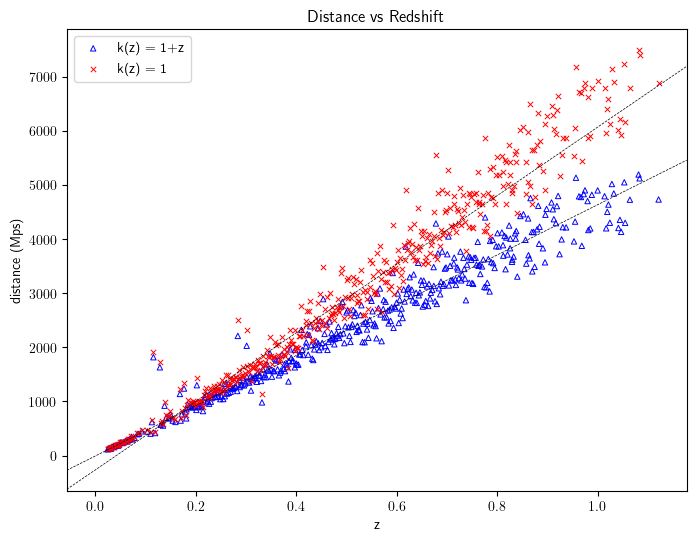
\includegraphics[width=\linewidth]{../graphs/mu_distance_vs_redshift.png}
  \caption{The relationship between distance and redshift for two treatments of
  magnitude data. The displayed points are roughly a third of the values in the
  full DES dataset, selected evenly to aid visibility. The $k(z) = 1$ treatment
  is clearly non-linear while the $k(z) = 1 + z$ treatment appears to be
  linear.}
  \label{fig:mu_distance_vs_redshift}
\end{figure}

\section{Disagreement with existing research}

Previous studies use $F$ instead of $F*$. To the best of our knowledge, no
studies that depend on the distance of Type Ia supernova, reaching back at
least to \citet{riess1998} and \citet{perlmutter1999}, have accounted for time
dilation.

\bibliographystyle{unsrtnat}
\bibliography{references}

\end{document}
